\documentclass[a4paper, 12pt]{article}		% general format
\usepackage{multicol}
%%%% Charset
\usepackage{cmap}							% make PDF files searchable and copyable
\usepackage[utf8x]{inputenc} 				% accept different input encodings
\usepackage[english,russian]{babel}   %% загружает пакет многоязыковой вёрстки
\usepackage{fontspec}      %% подготавливает загрузку шрифтов Open Type, True Type и др.
\defaultfontfeatures{Ligatures={TeX},Renderer=Basic}  %% свойства шрифтов по умолчанию
\setmainfont[Ligatures={TeX,Historic}]{Roboto-Light} %% задаёт основной шрифт документа
\setsansfont{Roboto-Light}  
\usepackage{float}
%%%% Graphics
\usepackage[dvipsnames]{xcolor}			% driver-independent color extensions
\usepackage{graphicx}						% enhanced support for graphics
\usepackage{wrapfig}						% produces figures which text can flow around

%%%% Math
\usepackage{amsmath}						% American Mathematical Society (AMS) math facilities
\usepackage{amsfonts}						% fonts from the AMS
\usepackage{amssymb}						% additional math symbols

%%%% Typograpy (don't forget about cm-super)
\usepackage{microtype}						% subliminal refinements towards typographical perfection
\linespread{1.3}							% line spacing
\usepackage[left=2.5cm, right=1.5cm, top=2.5cm, bottom=2.5cm]{geometry}
\setlength{\parindent}{0pt}					% we don't want any paragraph indentation
\usepackage{parskip}						% some distance between paragraphs

%%%% Tables
\usepackage{tabularx}						% tables with variable width columns
\usepackage{multirow}						% for tabularx
\usepackage{hhline}							% for tabularx
\usepackage{tabu}
\usepackage{longtable}

%%%% Graph
\usepackage{tikz}							% package for creating graphics programmatically
\usetikzlibrary{arrows}						% edges for tikz

%%%% Other
\usepackage{url}							% verbatim with URL-sensitive line breaks
\usepackage{fancyvrb}						% sophisticated verbatim text (with box)

\usepackage{listings}
\usepackage{caption}
\DeclareCaptionFont{white}{\color{white}}
\DeclareCaptionFormat{listing}{\colorbox{gray}{\parbox{\dimexpr\textwidth-1.72\fboxsep\relax}{#1#2#3}}}
\captionsetup[lstlisting]{format=listing,labelfont=white,textfont=white,margin=0pt}
\lstset{language=C,
	basicstyle=\footnotesize,
	keepspaces=true,
	tabsize=4,               
	frame=single,                           % Single frame around code
	rulecolor=\color{black},
	captionpos=b,
	showstringspaces=false,	
	abovecaptionskip=-0.9pt,
	xleftmargin=3.4pt,
	xrightmargin=2.6pt,
	breaklines=true,
	postbreak=\raisebox{0ex}[0ex][0ex]{\ensuremath{\color{black}\hookrightarrow\space}},
	xleftmargin=3.2pt,
	literate={а}{{\selectfont\char224}}1
	{~}{{\textasciitilde}}1
	{б}{{\selectfont\char225}}1
	{в}{{\selectfont\char226}}1
	{г}{{\selectfont\char227}}1
	{д}{{\selectfont\char228}}1
	{е}{{\selectfont\char229}}1
	{ё}{{\"e}}1
	{ж}{{\selectfont\char230}}1
	{з}{{\selectfont\char231}}1
	{и}{{\selectfont\char232}}1
	{й}{{\selectfont\char233}}1
	{к}{{\selectfont\char234}}1
	{л}{{\selectfont\char235}}1
	{м}{{\selectfont\char236}}1
	{н}{{\selectfont\char237}}1
	{о}{{\selectfont\char238}}1
	{п}{{\selectfont\char239}}1
	{р}{{\selectfont\char240}}1
	{с}{{\selectfont\char241}}1
	{т}{{\selectfont\char242}}1
	{у}{{\selectfont\char243}}1
	{ф}{{\selectfont\char244}}1
	{х}{{\selectfont\char245}}1
	{ц}{{\selectfont\char246}}1
	{ч}{{\selectfont\char247}}1
	{ш}{{\selectfont\char248}}1
	{щ}{{\selectfont\char249}}1
	{ъ}{{\selectfont\char250}}1
	{ы}{{\selectfont\char251}}1
	{ь}{{\selectfont\char252}}1
	{э}{{\selectfont\char253}}1
	{ю}{{\selectfont\char254}}1
	{я}{{\selectfont\char255}}1
	{А}{{\selectfont\char192}}1
	{Б}{{\selectfont\char193}}1
	{В}{{\selectfont\char194}}1
	{Г}{{\selectfont\char195}}1
	{Д}{{\selectfont\char196}}1
	{Е}{{\selectfont\char197}}1
	{Ё}{{\"E}}1
	{Ж}{{\selectfont\char198}}1
	{З}{{\selectfont\char199}}1
	{И}{{\selectfont\char200}}1
	{Й}{{\selectfont\char201}}1
	{К}{{\selectfont\char202}}1
	{Л}{{\selectfont\char203}}1
	{М}{{\selectfont\char204}}1
	{Н}{{\selectfont\char205}}1
	{О}{{\selectfont\char206}}1
	{П}{{\selectfont\char207}}1
	{Р}{{\selectfont\char208}}1
	{С}{{\selectfont\char209}}1
	{Т}{{\selectfont\char210}}1
	{У}{{\selectfont\char211}}1
	{Ф}{{\selectfont\char212}}1
	{Х}{{\selectfont\char213}}1
	{Ц}{{\selectfont\char214}}1
	{Ч}{{\selectfont\char215}}1
	{Ш}{{\selectfont\char216}}1
	{Щ}{{\selectfont\char217}}1
	{Ъ}{{\selectfont\char218}}1
	{Ы}{{\selectfont\char219}}1
	{Ь}{{\selectfont\char220}}1
	{Э}{{\selectfont\char221}}1
	{Ю}{{\selectfont\char222}}1
	{Я}{{\selectfont\char223}}1,
	extendedchars=true
}

%галочка
\usepackage{amssymb}% http://ctan.org/pkg/amssymb
\usepackage{pifont}% http://ctan.org/pkg/pifont
\newcommand{\cmark}{\ding{52}}%
\newcommand{\xmark}{\ding{56}}
%------------------------------------------------------------------------------
\renewcommand{\labelenumii}{\theenumii}
\renewcommand{\theenumii}{\theenumi.\arabic{enumii}.}
\begin{document}
%------------------------------------------------
	\begin{titlepage}
		\begin{center}
			\large {Санкт-Петербургский политехнический университет Петра Великого\\
				Институт компьютерных наук и технологий}\\
		\end{center}
		\begin{center}
			\large\textbf {Кафедра компьютерных систем и программных технологий}
		\end{center}
		\vfill
		\begin{center}
			\large{\textbf{Отчет о лабораторной работе №5} \\
			\textbf{Курс: } Администрирование компьютерных сетей\\
			\textbf{Тема: } Перенос сети в Cisco Packet Tracer}
		\end{center}
		
		\vfill
		
		\flushleft{Выполнил студент группы 13541/3} 
		\hfill\parbox{9 cm}{\hspace*{3cm}\hbox to 0cm{\raisebox{-1em}{\small(подпись)}}\hspace*{-0.8cm}\rule{3cm}{0.8pt} Д.В. Круминьш}\\[0.6cm]
		
		\flushleft{Преподаватель} \hfill\parbox{9 cm}{\hspace*{3cm}\hbox to 0cm{\raisebox{-1em}{\small(подпись)}}\hspace*{-0.8cm}\rule{3cm}{0.8pt} И.А. Малышев}\\[0.6cm]
		
		\vspace{\fill}
		\begin{center}
			Санкт-Петербург \\ 2018 г.
		\end{center}
	\end{titlepage}
%------------------------------------------------
\setcounter{page}{2}
%\tableofcontents
%\clearpage

%------------------------------------------------------------------------------
%\input{intro}
\section{Цели работы}
\begin{enumerate}
\item Изучение утилит и систем администрирования TCP/IP-сетей.
\item Мониторинг и анализ характеристик TCP/IP-сетей.
\end{enumerate}

\section{Сведения о системе}
Работа производилась на реальной системе, со следующими характеристиками:
\tabulinesep = 1mm
\begin{longtabu} to \textwidth {|X[10, c , m ] |X[25, c , m ] | }\firsthline\hline

\textbf{Элемент}&\textbf{Значение}\\ \hline \endfirsthead
	
Имя ОС&Майкрософт Windows 10 Pro (Registered Trademark)\\ \hline
Версия&10.0.16299 Сборка 16299\\ \hline
Установленная оперативная память (RAM) &16,00 ГБ\\ \hline
Процессор&Intel(R) Core(TM) i5-7300HQ CPU @ 2.50GHz, 2496 МГц, ядер: 4, логических процессоров: 4\\ \hline
\caption{Сведения о системе}
\end{longtabu}
Для выполнения работы использовалась \textbf{VMware Workstation 12 pro (12.5.7 build-5813279)}
В качестве сети для экспериментов, использовалась ККС из прошлой работы.

\section{Оценка пропускной способности}
В качестве утилиты для оценки пропускной способности была выбрана \textbf{iperf}.  Iperf — кроссплатформенная консольная клиент-серверная программа, предназначена для тестирования пропускной способности интернет канала между двумя компьютерами.

Измерение осуществляется следующим образом, на одном ПК запускаем iperf в режиме «сервер», на втором в режиме «клиент» с указанием ip-адреса первого ПК («сервера»). Через заданное время показывается измеренная информация. 

В работе использовалась \textbf{версия} 2.0.5
\subsection{Установка}
На \textbf{NetBsd}, были выполнены команды:
\begin{enumerate}
\item Загрузка iperf
\begin{enumerate}
\item Подключение к ftp серверу, к папке с пакетами для моей версии NetBSD
\begin{lstlisting}[language={}]
ftp -i ftp://ftp.netbsd.org/pub/pkgsrc/packages/NetBSD/x86_64/7.1.1/All/
\end{lstlisting}
\item Загрузка последней версии
\begin{lstlisting}[language={}]
mget iperf-2.0.5nb1.tgz
\end{lstlisting}
\item Завершение работы ftp
\begin{lstlisting}[language={}]
quit
\end{lstlisting}
\end{enumerate}
\item Создаем папку и разархивируем туда архив
\begin{lstlisting}[language={}]
mkdir iperf
tar -xzf iperf-2.0.5nb1.tgz -C /root/iperf
\end{lstlisting}
\item Утилита для запуска находится по пути \textbf{/root/iperf/bin}
\end{enumerate}

На \textbf{FreeBSD}, были выполнены команды:
\begin{lstlisting}[language={}]
cd /usr/ports/benchmarks/iperf
make install clean
\end{lstlisting}
На \textbf{Kali Linux}, была выполнена команда:
\begin{lstlisting}[language={}]
apt-get install iperf
\end{lstlisting}
На \textbf{Windows XP} были скачены бинарные файлы программы.

\subsection{Тестирование}
На хосте с FreeBSD запущен сервер iperf
\begin{lstlisting}[language={}]
iperf -s
\end{lstlisting}
На машинах(Kali Linux, NetBSD, Windows XP) iperf запущен в качестве клиента, командой:
\begin{lstlisting}[language={}]
iperf -c 192.168.40.2
\end{lstlisting}
В результате были получены следующие данные:
\tabulinesep = 1mm
\begin{longtabu} to \textwidth {|X[ c , m ] |X[c , m ] | X[ c , m ]|}\firsthline\hline
\textbf{NetBSD}&\textbf{Kali Linux}&\textbf{Windows XP}\\ \hline \endfirsthead
1.47 Гбит/c&1.62 Гбит/c&5.81 Мбит/c\\ \hline
\caption{Пропускная способность систем}
\end{longtabu}

\section{Карта сети}
Для изучения сети использована программа \textbf{10-Страйк: Схема Сети}(версия 3.32), установленная на Windows XP.

При запуске программы, были указаны следующие диапазоны для сканирования:
\begin{itemize}
\item 192.168.32.1-192.168.32.254;
\item 192.168.40.1-192.168.40.254;
\item 192.168.80.1-192.168-80.254;
\item 192.168.120.1-192.168.120.254.
\end{itemize}
В качестве параметров тестирования выбрать ICMP-ping. 

После чего начнется сканирование данных диапазонов адресов. Программа построила следующую карту сети:
\begin{figure}[H]
  \centering
  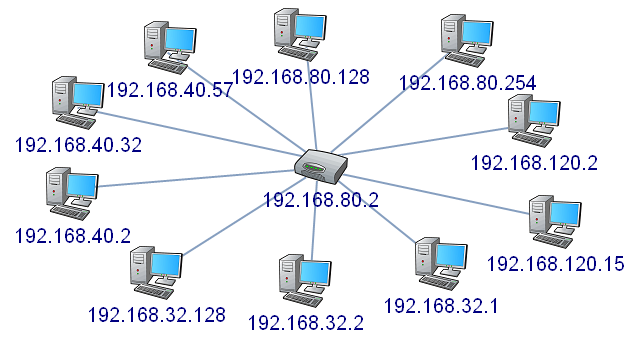
\includegraphics[width=.7\textwidth]{img/3}
  \caption{Карта сети}
\end{figure}
Программа не смогла определить точную карту сети, типы операционных систем, она видит лишь ближайший маршрутизатор, в данном случае – это FreeBSD (хост 192.168.80.2).
\section{Поиск уязвимостей}
В качестве программы по поиску уязвимостей была выбрана \textbf{X-Spider}(версия 7.7), которая была установлена на Windows XP.

Перед сканированием были добавлены следующие адреса интерфейсов:
\begin{multicols}{2}
\begin{itemize}
\item 192.168.80.128(Windwos XP);
\item 192.168.40.2(FreeBSD);
\item 192.168.80.2(FreeBSD);
\item 192.168.120.2(FreeBSD);
\item 192.168.120.15(Windows 98);
\item 192.168.40.32(Kali Linux);
\item 192.168.40.57(NetBSD);
\item 192.168.32.128(NetBSD).
\end{itemize}
\end{multicols}

По итогам работы, были выявлены следующие уязвимости:
\begin{itemize}
\item Windows XP
\begin{itemize}
\item имя операционной системе;
\item сервисом NTP открыт порт 123 по UDP;
\item сервисом RPC Windows открыт порт 135 по TCP;
\item сервисом NBNS открыт порт 137 по UDP;
\item сервисом NetBIOS открыт порт 139 по TCP.
\end{itemize}
\item Windows 98
\begin{itemize}
\item имя операционной системе;
\item сервисом NetBIOS-SSN открыт порт 137 по UDP;
\item сервисом NetBIOS открыт порт 139 по TCP.
\end{itemize}
\end{itemize}
В системах unix слабых мест не обнаружено.
\section*{Вывод}
В результате выполнения данной лабораторной работы была протестирована сеть на основе TCP/IP. 

Оценка пропускной способности показала свехвысокую скорость для ос семейства unix и весьма медленную для windows xp. Возможно это связано с кроссплатформенностью утилиты для тестирования и различных настроек операционных систем.

Утилита для построения карты сети, показала некорректную карту сети, что о говорит о сложности построения реальной карты сети.

Тестирование на уязвимости показало, что уязвимостям подвержены ОС семейства Windows, в то время как на unix системах уязвимостей найдено не было.

Для предотвращения подобных уязвимостей, необходимо использовать операционные системы актуальных версий(с последними обновлениями). Также желательно наличие какого-либо специализированного ПО для защиты системы.
%------------------------------------------------------------------------------

%\addcontentsline{toc}{section}{Список литературы}
%\bibliography{thesis}
%\bibliographystyle{ugost2008}

\end{document}